\documentclass[11pt,a4paper]{jarticle}
\usepackage[dvipdfmx]{graphicx}
\usepackage{url}

\renewcommand{\baselinestretch}{1.05} 
\marginparwidth=0cm
\topmargin=-1cm
\headheight=0.3cm
\headsep=0.7cm
\oddsidemargin=0cm
\evensidemargin=0cm
%\textwidth=43zw
\textwidth=15.92cm
%\textheight=43.3\baselineskip
\baselineskip = 0.5744cm
\textheight=43\baselineskip

\itemsep=0.05\baselineskip
\parsep=0pt
\topsep=0.01\baselineskip
\partopsep=0pt
\listparindent=0zw

%% header and footer
\usepackage{fancyhdr}
\pagestyle{fancy}
\lhead{2014年度 春学期授業}
\chead{インタラクティブ・アート実習}
\rhead{担当教員: 松下 光範}
\cfoot{\thepage}
\renewcommand{\headrulewidth}{0pt}
\renewcommand{\footrulewidth}{0pt}

\usepackage{ascmac}
\usepackage{listings,jlisting}
\usepackage{color}
\definecolor{OliveGreen}{cmyk}{0.64,0,0.95,0.40}
\definecolor{colFunc}{rgb}{1,0.07,0.54}
\definecolor{CadetBlue}{cmyk}{0.62,0.57,0.23,0}
\definecolor{Brown}{cmyk}{0,0.81,1,0.60}
\definecolor{colID}{rgb}{0.63,0.44,0}
\definecolor{rulesepcolor}{gray}{0.666}
\lstset{
  language=Java,%プログラミング言語によって変える。
  basicstyle={\ttfamily\small},
  keywordstyle={\color{OliveGreen}},
  %[2][3]はプログラミング言語によってあったり、なかったり
  keywordstyle={[2]\color{colFunc}},
  keywordstyle={[3]\color{CadetBlue}},%
  commentstyle={\color{Brown}},
  %identifierstyle={\color{colID}},
  stringstyle=\color{blue},
  tabsize=2,
  %frame=trBL,
  %numbers=left,
  numberstyle={\ttfamily\small},
  breaklines=true,%折り返し
  %backgroundcolor={\color[gray]{.95}},
  framexleftmargin=0mm,
  frame=single,
  rulesepcolor=\color{rulesepcolor},
  captionpos=b
}


%%%%%%%%%%%%%%%%%%%%%%%%%%%%%%%%%%%%%%%%%%%%%%%%%%%%%%%%%%%%%%%%
\begin{document}
% title
\section*{\LARGE{第4講 Analog Output を用いて LED を制御する}}
%%%%%%%%%%%%%%%%%%%%%%%%%%%%%%%%%%%%%%%%%%%%%%%%%%%%%%%%%%%%%%%%

\section{Analog Output}
前回までは、Digital Input と Digital Output を用いて、
スイッチの ON/OFF を取得したり、 LED を点滅させたりしました。
しかし、単に ON/OFF を取得するのではなくもう少し緩やかな変化を取得したい場合や、
LED をじわじわと光らせたい場合などがあると思います。
そのような場合には Digital Input/Output ではなく Analog Input/Output を使います。

今回は Analog Output を用いて、LED を任意の明るさで光らせる、ということをやってみましょう。

\subsection*{PWM (Pulse Width Modulation)}
実は、Arduino においての Analog Output は実際に電圧が変化するのではなく、
PWM (Pulse Width Modulation) と呼ばれる方式で擬似的に実現しています。

Processing から Arduino の Analog Output を用いるためには準備として、
\begin{lstlisting}
 // pinNum は回路に合わせて変える 
 arduino.pinMode(pinNum, Arduino.OUTPUT);
\end{lstlisting}
が必要となります。
これは Digital Output のときと同様です。

Digital Output のときは arduino.digitalWrite() を用いましたが、
Analog Output の場合は
\begin{lstlisting}
 // value は 0〜255 で設定
 arduino.analogWrite(pinNum, value);
\end{lstlisting}
を用います。
Digital Output のときは、Arduino.HIGH (5V) か Arduino.LOW (0V) のどちらかにしましたが、
Analog Output の場合は 0〜255 の値で自由に設定できます。
これにより、緩やかに LED の明るさを変化させるといったことが可能になります。

\section{LED を徐々に光らせる}
では、Analog Output を用いて実際に LED の光り方を細かく制御してみましょう。

\subsection*{mouseX と mouseY}
ついでに Processing の新しい命令を覚えましょう。
前回の実習で、マウスボタンの ON/OFF (true/false) を mousePressed 変数で取得できることを学びました。
今回はボタンを押したかどうかではなく、マウスポインタの座標を取得してみましょう。
マウスポインタの x 座標と y 座標を取得するためにはそれぞれ mouseX 変数と mouseY 変数を用います。

\subsubsection*{サンプルプログラム}
\begin{lstlisting}
 void setup() {
   size(256, 256);
 }

 void draw() {
   background(0);
   // マウスポインタの座標に円を描く
   ellsepse(mouseX, mouseY, 32, 32);
 }
\end{lstlisting}

今回は、 mouseX、mouseY の値によって LED の明るさを変化させる、ということをやってみます。

回路は前回とほとんど同じで OK ですが、接続するピンに注意してください (ledPin を自分の回路で用
いてるピンと置き換える)。
また、PWM を用いる場合は、番号の前に ''$\sim$'' が付いているピン ($\sim9$ とか) を用いてください。こちらにも注意!


\subsection*{プログラム}
\begin{lstlisting}
 import processing.serial.*;
 import cc.arduino.*;
 
 Arduino arduino;
 int ledPin = 9;   // LEDが接続されたピン番号

 void setup() {
   size(256, 256);
   arduino = new Arduino(this, Arduino.list()[6], 57600);
   arduino.pinMode(ledPin, Arduino.OUTPUT);
 }

void draw() {
  // マウスのx座標をLEDの明るさにする 
  arduino.analogWrite(ledPin, mouseX);
}
\end{lstlisting}

\subsection*{回路}
\begin{figure}[h!]
 \centering
 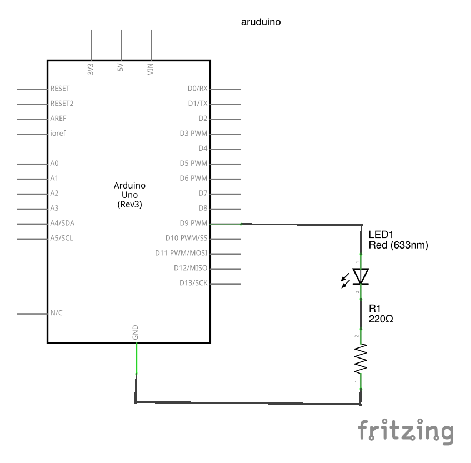
\includegraphics[width=0.5\columnwidth]{img/LED_circuit.eps}
 \caption{LEDのフェードインとフェードアウトの回路図}
\end{figure}

\section{フルカラー LED}
フルカラー LED を用いると、光の三原色をそれぞれ制御することによって、様々の色の表現が可能となります。
フルカラー LED の構造は単純で、内部に赤、緑、青の3つのLEDが入っていると考えれば良いです。
そのため、単色 LED のときは光り方を制御するために 1 つの Output を用いましたが、
フルカラー LED の場合は 3 色をそれぞれ制御する必要があるため 3 つの Analog Output を用います。
また、端子が 4 本出ているものが多いですが、これはアノード(+)またはカソード(-)が3つ分共通になっているためで、それぞれアノードコモン、カソードコモンと呼びます。

\begin{figure}[h!]
 \begin{minipage}{0.35\columnwidth}
  \centering
  \includegraphics[height=40mm]{img/full_color_led_detail.eps}
  \caption{フルカラー LED}
 \end{minipage}
 \begin{minipage}{0.65\columnwidth}
  本実習では、カソードコモンのものを用いる。% 要確認
  それぞれの端子は
  \begin{itemize}
   \item[R:] 赤
   \item[G:] 緑
   \item[B:] 青
   \item[K:] - (カソード)
  \end{itemize}
  に対応する。
  順番に注意すること!
 \end{minipage}
\end{figure}

\subsection*{プログラム}
\begin{lstlisting}
import processing.serial.*;
import cc.arduino.*;
 
Arduino arduino;
int LED_R = 9;    // LED 赤
int LED_B = 10;   // LED 青
int LED_G = 11;   // LED 緑

void setup() {
  size(256, 256);
  arduino = new Arduino(this, Arduino.list()[6], 57600);
  //LEDのピンを出力に設定する
  arduino.pinMode(LED_R, Arduino.OUTPUT);
  arduino.pinMode(LED_B, Arduino.OUTPUT);
  arduino.pinMode(LED_G, Arduino.OUTPUT);
}

void draw() {
  // LEDの明るさをセット
  arduino.analogWrite(LED_R, mouseX);
  arduino.analogWrite(LED_B, mouseY);
  arduino.analogWrite(LED_G, 127);
}
\end{lstlisting}

\subsection*{回路}
\begin{figure}[h!]
 \begin{minipage}{0.5\columnwidth}
  \centering
  \includegraphics[height=60mm]{img/Full_color_LED.eps}
  \caption{フルカラーLEDの配線図}
  \label{circuit}
 \end{minipage}
 \begin{minipage}{0.5\columnwidth}
  \centering
  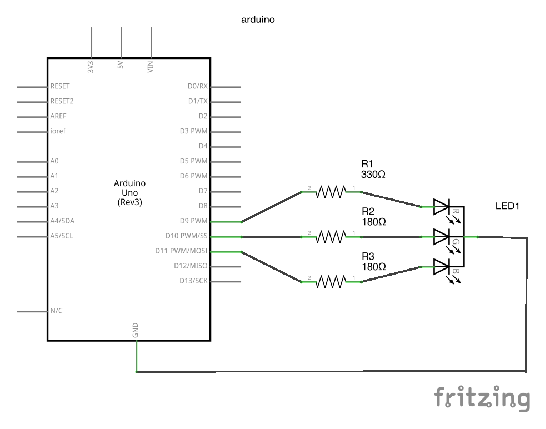
\includegraphics[height=60mm]{img/Full_color_LED_circuit.eps}
  \caption{フルカラーLEDの回路図}
 \end{minipage}
\end{figure}

\end{document}